\documentclass{beamer}
\usetheme{Madrid}
\usepackage{amsmath}
\usepackage{graphicx}
\usepackage{mathrsfs}
\usepackage{tikz}
\usepackage{color}
\usepackage{bm}
\usepackage{subfigure}
\usetikzlibrary{bayesnet}
\DeclareMathOperator*{\argmax}{arg\,max}
\newcommand*\diff{\mathop{}\!\mathrm{d}}
\newcommand*\Diff[1]{\mathop{}\!\mathrm{d^#1}}
\title{Nonparametric Bayesian Models}
\author{Jie Tang}

\begin{document}

\begin{frame}
\titlepage
\end{frame}

\begin{frame}
\frametitle{Outline}
\tableofcontents[pausesections]
\end{frame}

\section{Introduction}
\begin{frame}
	\frametitle{Introduction}
	\begin{itemize}
		\item We'll talk about {\em nonparametric Bayesian methods} in following slides
		\begin{itemize}
			\item Regression, classification -- Gaussian Process
			\item Clustering -- Dirichlet Process
		\end{itemize}
		\item What is {\em nonparametric} ?
		\item What is {\em Bayesian} ?
	\end{itemize}
\end{frame}

\begin{frame}
	\frametitle{What is Nonparametric Model?}
	\begin{itemize}
		\item Nonparametric doesn't mean there are no parameters.
		\item {\color{red} Parametric} model assumes a finite set of parameters.
		\begin{itemize}
			\item Finite model parameters captures everything about the data
			\item Predictions for future data are made merely through parameters, independent from observed data.			
			\item Model complexity are bounded, even with infinite data 	
		\end{itemize}
		\item {\color{red} Nonparametric} model assumes the model can't be specified by a finite set of parameters. But often a infinite-dimensional parameter space will work.
		\begin{itemize}
			\item Model complexity can grow with data
		\end{itemize}
	\end{itemize}
\end{frame}

\begin{frame}
	\frametitle{Example: Classification}
	\begin{itemize}
		\item{Consider a linear model}
		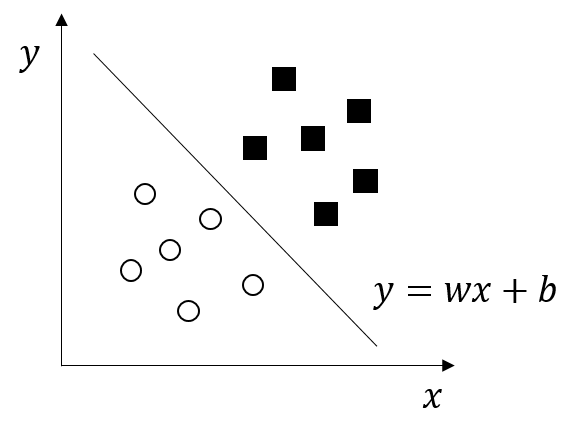
\includegraphics[width=0.6\textwidth]{img/linear.png}
		\item{No matter how many samples are trained, number of parameters are fixed $(w,b)$}
	\end{itemize}
\end{frame}

\begin{frame}
	\frametitle{Example: Classification}
	\begin{itemize}
		\item{How about k-NN?}
		\item 2 samples
		\begin{figure}	
		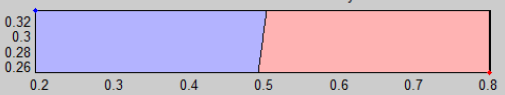
\includegraphics[width=0.6\textwidth]{img/knn2.png}
		\end{figure}
	\end{itemize}
\end{frame}

\begin{frame}
	\frametitle{Example: Classification}
	\begin{itemize}
		\item 10 samples
		\begin{figure}		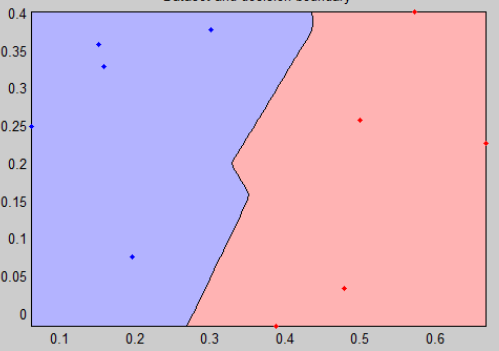
\includegraphics[width=0.6\textwidth]{img/knn10.png}
		\end{figure}
		
	\end{itemize}
\end{frame}
\begin{frame}
	\frametitle{Example: Classification}
	\begin{itemize}
		\item 100 samples
		\begin{figure}	
		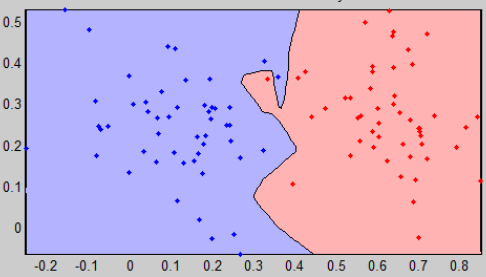
\includegraphics[width=0.6\textwidth]{img/knn100.png}
		\end{figure}
		\item Parameters are unbounded as dataset grow larger
		\item Nonparametric!
	\end{itemize}
\end{frame}

\begin{frame}
	\frametitle{What about SVM?}
	\begin{itemize}
		\item {Linear SVM}
		\[
			y=\text{sign}(w^Tx)
		\]
		\pause
		\item {Kernel SVM}
		\[
			y=\text{sign}(\sum_i \alpha_i y_i\kappa(x_i, x)))
		\]
	\end{itemize}
\end{frame}
\begin{frame}
	\frametitle{Parametric vs. Nonparametric}
	\begin{itemize}
		\item Parametric Models:
		\begin{itemize}
			\item Inflexible. Simple and easy to interpret.
			\item Performs well and fast, if model captures the data correctly
			\item Otherwise will give inconsistent result
		\end{itemize}
		\item Nonparametric Models:
		\begin{itemize}
			\item Flexible.
			\item Complex and hard to interpret, thus giving inaccurate estimation
		\end{itemize}
	\end{itemize}
\end{frame}

\begin{frame}
	\frametitle{What is Bayesian?}
	\begin{itemize}
		\item Consider a regression problem
		\item Given training data $D$, we aim to find a model $f$. For each sample $x$, return a prediction $y$
		\item How to give an optimal $y$?
		\begin{itemize}
			\pause
			\item MLE
			\item MAP
			\item Bayesian
		\end{itemize}
	\end{itemize}
\end{frame}
\begin{frame}
	\frametitle{Maximum Likelihood Estimation}
	\begin{itemize}
		\item In training, we maximize a likelihood
		\[
			f^* = \argmax_f L(f|D) = \argmax_f p(D|f)
		\]
		\item In prediction, just feed $f$ with $x$
		\[
			p(y|x, D)=p(y|f^*, x)
		\]
	\end{itemize}
\end{frame}
\begin{frame}
	\frametitle{Maximum A Posteriori}
	\begin{itemize}
		\item To avoid overfitting, we place a prior on the model
		\[
			f^* = \argmax_f \frac{p(D|f)p(f)}{p(D)}
		\]
		\item Prediction process remains the same
		\[
			p(y|x, D)=p(y|f^*, x)
		\]
	\end{itemize}
\end{frame}
\begin{frame}
	\frametitle{Bayesian Model}
	\begin{itemize}
		\item In training, we just estimate the posterior distribution of $f$ (same as MAP)
		\[
			p(f|D) = \frac{p(D|f)p(f)}{p(D)}
		\]
		\item In prediction, we no longer want a pointwise estimation. Instead, we consider all possible models and take the expection
		\[
			p(y|x, D)=\int_f p(y|f,x)p(f|D)\diff f
		\]
	\end{itemize}
\end{frame}
\begin{frame}
	\frametitle{Why Bayesian?}
	\begin{itemize}
		\item Infinite Exchangeability:
		\[
		\forall n, \forall \sigma, p(x_1, \ldots, x_n)=p(x_{\sigma(1)},\ldots, x_{\sigma(n)})
		\]
		\item De Finetti’s Theorem: If $(x_1, x_2, \ldots)$ are infinite exchangable, then there exists a random variable $f$, $\forall n$, 
		\[
		p(x_1, \ldots, x_n) = \int_{f} \prod_{i=1}^n p(x_i|f)p(f) \diff f
		\]
		\pause
		\item \em{How to define the prior $p(f)$}?
	\end{itemize}		
\end{frame}

\begin{frame}
	\frametitle{Parametric Approach}
	\begin{itemize}
		\item In previous courses, we focused on parametric representation of $f$, e.g.
		\[
			f(x)=w^Tx
		\]
		\item Instead of defining prior on function itself, we define prior on the parameters
		\[
			p(w) = \mathcal{N}(0, \sigma^2 I)
		\]
		\item Now, we define the prior on the function $f$ directly
	\end{itemize}	
\end{frame}

\section{Gaussian Process}
\subsection{Multivariate Gaussian Distribution}
\begin{frame}
	\frametitle{Warmup: Multivariate Gaussian}
	\begin{itemize}
		\item Before introducing Gaussian Process, let's recall multivariate Gaussian distribution first.
		\item We say a $n$-dimensional random variable $\mathbf{x}$ follows multivariate Gaussian 
			\[
				 \bm{x} \sim \mathcal{N}(\bm{\mu}, \bm{\Sigma})
			\]
			if
			\[
				p(\bm{x}) = \frac{1}{{\sqrt {{{(2\pi )}^n}{\rm{|}}\bm{\Sigma} {\rm{|}}} }}\exp \{  - \frac{1}{2}{(\bm{x-\mu})^T}{\bm{\Sigma} ^{ - 1}}({\bm{x - \mu}})\}
			\]
			where
			\begin{align*}
				& \mathbb{E}[\mathbf{x}] = \bm{\mu} \\
				& \mathbb{E}[(x_i-\mu_i)(x_j-\mu_j)] = \Sigma_{ij}
			\end{align*}
	\end{itemize}
\end{frame}

\begin{frame}
	\frametitle{Marginal Distribution}
	\begin{itemize}
		\item Suppose

		\[\left[ {\begin{array}{*{20}{c}}
			{\bm{x_1}}\\
			{\bm{x_2}}
			\end{array}} \right] \sim \mathcal{N}\left( {\left[ {\begin{array}{*{20}{c}}
				{\bm{\mu _1}}\\
				{\bm{\mu _2}}
				\end{array}} \right],\left[ {\begin{array}{*{20}{c}}
				{\bm{\Sigma _{11}}}&{\bm{\Sigma _{12}}}\\
				{\bm{\Sigma _{21}}}&{\bm{\Sigma _{22}}}
				\end{array}} \right]} \right)\]

		\item Integrating $\bm{x_2}$ out, 
		\[
			\bm{x_1} \sim \mathcal{N}(\bm{\mu_1}, \bm{\Sigma_{11}})
		\]
		\item Just drop irrelevant components
	\end{itemize}
\end{frame}

\begin{frame}
	\frametitle{Contitional Distribution}
	\begin{itemize}
		\item Suppose
		
		\[\left[ {\begin{array}{*{20}{c}}
			{\bm{x_1}}\\
			{\bm{x_2}}
			\end{array}} \right] \sim \mathcal{N}\left( {\left[ {\begin{array}{*{20}{c}}
				{\bm{\mu _1}}\\
				{\bm{\mu _2}}
				\end{array}} \right],\left[ {\begin{array}{*{20}{c}}
				{\bm{\Sigma _{11}}}&{\bm{\Sigma _{12}}}\\
				{\bm{\Sigma _{21}}}&{\bm{\Sigma _{22}}}
				\end{array}} \right]} \right)\]
		\item Then
		\begin{align*}
			p(\bm{x_1|x_2}) &= \mathcal{N}(\bm{x_1|\mu_{1|2}, \Sigma_{1|2}}) \\
			\bm{\mu_{1|2}} & = \bm{\mu _1 + \Sigma _{12}\Sigma _{22}^{ - 1}({x_2}{\rm{ - }}{\mu _2})} \\
			\bm{\Sigma_{1|2}} & = \bm{\Sigma _{11} - \Sigma _{12}\Sigma _{22}^{ - 1}\Sigma _{21}}
		\end{align*}
		\item{We will use it later}
		\item{How to get that?}
	\end{itemize}
\end{frame}

\begin{frame}
	\frametitle{Some Detail}
	First, we diagonalize the variance matrix to ease the inverse matrix calculation
	\[\left[ {\begin{array}{*{20}{c}}
	{{\Sigma _{11}}/{\Sigma _{22}}}&O\\
	O&{{\Sigma _{22}}}
	\end{array}} \right] = \left[ {\begin{array}{*{20}{c}}
	{{I_1}}&{ - {\Sigma _{12}}\Sigma _{22}^{ - 1}}\\
	O&{{I_2}}
	\end{array}} \right]\left[ {\begin{array}{*{20}{c}}
	{{\Sigma _{11}}}&{{\Sigma _{12}}}\\
	{{\Sigma _{21}}}&{{\Sigma _{22}}}
	\end{array}} \right]\left[ {\begin{array}{*{20}{c}}
	{{I_1}}&O\\
	{ - \Sigma _{22}^{ - 1}{\Sigma _{21}}}&{{I_2}}
	\end{array}} \right]\]
	Define ${\Sigma _{11}}/{\Sigma _{22}} = {\Sigma _{11}} - {\Sigma _{12}}\Sigma _{22}^{ - 1}{\Sigma _{21}}$.
	Then
	\[
	\begin{split}
	{\left[ {\begin{array}{*{20}{c}}
			{{\Sigma _{11}}}&{{\Sigma _{12}}}\\
			{{\Sigma _{21}}}&{{\Sigma _{22}}}
			\end{array}} \right]^{ - 1}} = & \left[ {\begin{array}{*{20}{c}}
		{{I_1}}&O\\
		{ - \Sigma _{22}^{ - 1}{\Sigma _{21}}}&{{I_2}}
		\end{array}} \right] \\
		& \left[ {\begin{array}{*{20}{c}}
		{{{({\Sigma _{11}}/{\Sigma _{22}})}^{ - 1}}}&O\\
		O&{\Sigma _{22}^{ - 1}}
		\end{array}} \right]\left[ {\begin{array}{*{20}{c}}
		{{I_1}}&{ - {\Sigma _{12}}\Sigma _{22}^{ - 1}}\\
		O&{{I_2}}
		\end{array}} \right]
	\end{split}
	\]
\end{frame}
\begin{frame}
	\frametitle{More Detail}
	Check the exponent of $p(\bm{x_1, x_2})$:
	
\[\arraycolsep=1.4pt\def\arraystretch{1.2}
\begin{array}{l}
\quad ({x_1} - {\mu _1},{x_2} - {\mu _2}){\left[ {\begin{array}{*{20}{c}}
		{{\Sigma _{11}}}&{{\Sigma _{12}}}\\
		{{\Sigma _{21}}}&{{\Sigma _{22}}}
		\end{array}} \right]^{ - 1}}\left( {\begin{array}{*{20}{c}}
	{{x_1} - {\mu _1}}\\
	{{x_2} - {\mu _2}}
	\end{array}} \right)\\
= {\left( {\begin{array}{*{20}{c}}
		{{x_1} - {\mu _1}}\\
		{{x_2} - {\mu _2}}
		\end{array}} \right)^T}\left[ {\begin{array}{*{20}{c}}
	{{I_1}}&O\\
	{ - \Sigma _{22}^{ - 1}{\Sigma _{21}}}&{{I_2}}
	\end{array}} \right]\left[ {\begin{array}{*{20}{c}}
	{{{({\Sigma _{11}}/{\Sigma _{22}})}^{ - 1}}}&O\\
	O&{\Sigma _{22}^{ - 1}}
	\end{array}} \right]\\
\qquad \left[ {\begin{array}{*{20}{c}}
	{{I_1}}&{ - {\Sigma _{12}}\Sigma _{22}^{ - 1}}\\
	O&{{I_2}}
	\end{array}} \right]\left( {\begin{array}{*{20}{c}}
	{{x_1} - {\mu _1}}\\
	{{x_2} - {\mu _2}}
	\end{array}} \right)\\
	= {({x_1} - {\mu _1} - {\Sigma _{12}}\Sigma _{22}^{ - 1}({x_2} - {\mu _2}))^T}{({\Sigma _{11}}/{\Sigma _{22}})^{ - 1}}\\
\qquad({x_1} - {\mu _1} - {\Sigma _{12}}\Sigma _{22}^{ - 1}({x_2} - {\mu _2})) + C
	\end{array}
	\]
Note that $p(\bm{x_1|x_2}) = \frac{p(\bm{x_1, x_2})}{p(\bm{x_2})}$, and $C$ is just the exponent of $p(\bm{x_2})$. From the equation we can get the mean and variance of the conditional distribution.	
\end{frame}
	
\subsection{Definition}
\begin{frame}
	\frametitle{Gaussian Process}
	\begin{itemize}
		\item Gaussian Process is a generalization of multivariate Gaussian to infinite variables -- {\em stochastic process}
		\item $\forall \mathbf{x_1}, \ldots, \mathbf{x_n}, (f(\mathbf{x_1}), \ldots, f(\mathbf{x_n}))$ is jointly Gaussian
		\item A Gaussian Process is fully specified by mean function $m(x)$ and covariance $\kappa(\mathbf{x}, \mathbf{x'})$
		\begin{align*}
				m(\mathbf{x}) &= \mathbb{E}[f(\mathbf{x})] \\
				\kappa(\mathbf{\mathbf{x}}, \mathbf{\mathbf{x'}}) &= \mathbb{E}[(f(\mathbf{x})-m(\mathbf{x}))(f(\mathbf{x'})-m(\mathbf{x'}))]				
		\end{align*}	
		Then, 
		\[
			 (f(\mathbf{x_1}), f(\mathbf{x_2}), \ldots, f(\mathbf{x_n}))^T \sim \mathcal{N}(\bm{\mu}, \bm{K})			 
		\]
		where
		\[
			\mu_i = m(\mathbf{x_i}), K_{ij} = \kappa(\mathbf{x}_i, \mathbf{x}_j)
		\]
		\item We require $\kappa$ to be a positive definite kernel.
	\end{itemize}
\end{frame}
\subsection{GP regression}
\begin{frame}
	\frametitle{GP Regression with noise-free observations}
	\begin{itemize}
			\item For simplicity, let's start with predictions using noise free observations
			\item Training set $D=\{(x_i, f_i)\}$, where $f_i=f(x_i)$
				\begin{itemize}
					\item Noise free! -- No uncertainty.
				\end{itemize}
			\item Test set $\mathbf{X_*}$. We want to predict outputs $f_*$
			\item From definition of GP,
		\[\left( {\begin{array}{*{20}{c}}
			\bm{f}\\
			{\bm{f_*}}
			\end{array}} \right)\sim \mathcal{N}\left( {\left( {\begin{array}{*{20}{c}}
			\bm{\mu} \\
			{\bm{\mu _*}}
			\end{array}} \right),\left[ {\begin{array}{*{20}{c}}
			\bm{K}&{\bm{K_*}}\\
			\bm{K_*^T}&{\bm{K_{**}}}
			\end{array}} \right]} \right)\]
	\end{itemize}
\end{frame}

\begin{frame}
	\frametitle{GP Regression with noise-free observations}
	\begin{itemize}
		\item Using results of marginal multivariate Gaussian,
		\begin{align*}
		 p(\bm{f_*|X_*,X,f}) & = \mathcal{N}(\bm{\mu_*, \Sigma_*}) \\
		 \bm{\mu_*} & = \bm{\mu(X_*)}+\bm{K}_*^T \bm{K}^{-1}(\bm{f-\mu(X)}) \\
		 \bm{\Sigma_*} & = \bm{K}_{**}-\bm{K}_*^T\bm{K}^{-1}\bm{K}_*
		\end{align*}
		\item We usually set $\mu(\bm{x})=0$, because GP can model the mean arbitrarily well.		
	\end{itemize}
\end{frame}
\begin{frame}
	\frametitle{Visualization}
	\begin{itemize}
		\item Let's see some samples from GP prior and posterior.
		\begin{figure}
			\subfigure[prior]{
				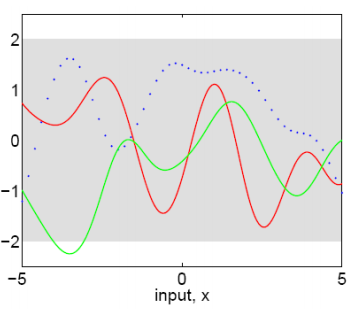
\includegraphics[width=0.3\columnwidth]{img/gp.png}
			}
			\subfigure[posterior]{
				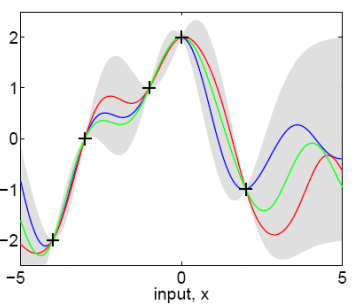
\includegraphics[width=0.3\columnwidth]{img/gp_posterior.png}
			}
		\end{figure}
		\item {Training data points are marked with '+'}.
		\item {No uncertainty at training data. Why?}
		\pause
		\item ${\bm{\Sigma_*}=\bm{K}_{**}-\bm{K}_*^T\bm{K}^{-1}\bm{K}_*}=0$ when $\bm{K_*}$ and $\bm{K}_{**}$ are sub-matrices of $\bm{K}$ -- Noise-free
	\end{itemize}
\end{frame}
\begin{frame}
	\frametitle{GP Regression with noisy observations}
	\begin{itemize}
		\item When observations are noisy, the true $f$ is hidden.
		\item Instead, we observe $f$ plus a Gaussian noise 
			\[
				y=f(\bm{x})+\epsilon
			\]
			where\[
			\epsilon \sim \mathcal{N}(0, \sigma_y^2)
			\]
		\item Now \[
		\text{cov}[y_p, y_q] = \kappa(\bm{x_p, x_q})+\sigma_y^2\delta_{pq}
		\] in other words
		\[
		\text{cov}[\bm{y|X}] = \bm{K}+\sigma_y^2 \bm{I} \triangleq \bm{K}_y
		\]
	\end{itemize}
\end{frame}
\section{Dirichlet Process}
\begin{frame}
	\frametitle{Example: Clustering}
	\begin{itemize}
		\item We're give a data set which are generated by a mixture of Gaussian.
		\item How to model the data and cluster them?
	\end{itemize}
	\centering
	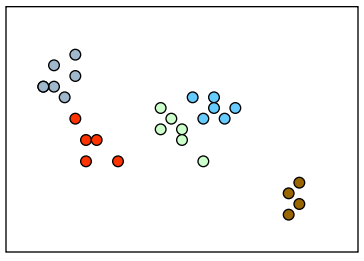
\includegraphics[width=0.6\textwidth]{img/motive.png}
\end{frame}

\begin{frame}
	\frametitle{Gaussian Mixture Clustering}
	
	\begin{columns}
		\column{0.6\textwidth}
		\begin{itemize}
			
			\item Suppose the dataset is generated by $K$ Gaussian components 
			\item Generating process:
			\begin{align*}
			\phi_k = (\mu_k, \Sigma_k) & \sim \mathcal{NIW}(\nu) \\
			\pi & \sim \text{Dirichlet}(\alpha/K, \ldots, \alpha/K) \\
			z_i & \sim \text{Multinomial}(\pi) \\
			x_i & \sim \mathcal{N}(\mu_{z_i}, \Sigma_{z_i})
			\end{align*}
			where 
			\begin{align*}
			\mathcal{NIW}(\nu) & : \text{conjugate prior of Gaussian} \\
			Dirichlet(\ldots) & : \text{conjugate prior of multinomial} \\
			z_i & : \text{mixture indicator of } x_i
			\end{align*}
		\end{itemize}
		\column{0.4\textwidth}
		\centering
		\tikz{ %
			
			\node[const] (alpha) {$\alpha$} ;
			\node[latent, below=of alpha] (pi) {$\pi$} ; 
			\node[latent, below=of pi] (z) {$z_i$} ;
			\node[obs, below=of z] (x) {$x_i$} ;        
			
			
			\node[latent, right=of z] (phi) {$\phi_k$} ; %
			\node[const, above=of phi] (nu) {$\nu$} ; %
			
			\edge{nu}{phi} ;
			\edge{alpha}{pi} ;
			\edge{pi}{z} ;
			\edge{z}{x} ;
			\edge{phi}{x} ;
			\plate[inner sep=0.25cm, xshift=-0.12cm, yshift=0.12cm]{plate1}{(z)(x)}{$i$} ;
			\plate[inner sep=0.25cm, xshift=-0.12cm, yshift=0.12cm]{plate2}{(phi)}{$k$} ;
		}
	\end{columns}
\end{frame}

\begin{frame}
	\frametitle{How to choose K?}
	\begin{itemize}
		\item How many clusters?
		\begin{center}
			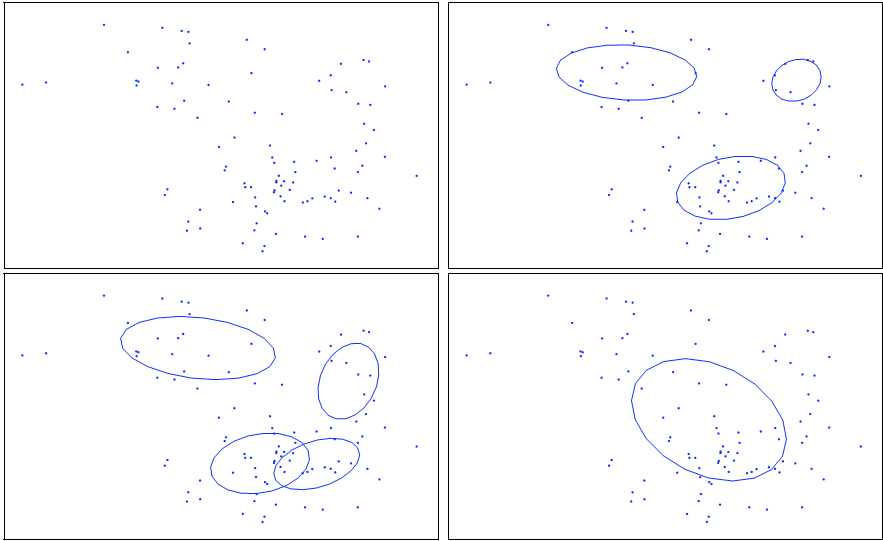
\includegraphics[width=0.6\textwidth]{img/unknown.png}
		\end{center}		
		\pause 
		\item What if let $K \rightarrow \infty$?
	\end{itemize}
\end{frame}

\begin{frame}
	\frametitle{Infinity Mixture Models}	
\begin{columns}
	\column{0.6\textwidth}
	\begin{itemize}
		\item Imagine $K\gg 0$, 
		\item In Bayesian inference, we integrate $\phi_k$ and $\pi$ out. Number of latent variables doesn't grow with $K$ -- No overfitting
		\item At most $n$ {\em active} components are associated with data
		\item It's an {\em infinite mixture model}
		\item Issue: can we take $K \rightarrow \infty$? What's the limiting model?
	\end{itemize}
	\column{0.4\textwidth}
	\centering
	\tikz{ %
		
		\node[const] (alpha) {$\alpha$} ;
		\node[latent, below=of alpha] (pi) {$\pi$} ; 
		\node[latent, below=of pi] (z) {$z_i$} ;
		\node[obs, below=of z] (x) {$x_i$} ;        
		
		
		\node[latent, right=of z] (phi) {$\phi_k$} ; %
		\node[const, above=of phi] (nu) {$\nu$} ; %
		
		\edge{nu}{phi} ;
		\edge{alpha}{pi} ;
		\edge{pi}{z} ;
		\edge{z}{x} ;
		\edge{phi}{x} ;
		\plate[inner sep=0.25cm, xshift=-0.12cm, yshift=0.12cm]{plate1}{(z)(x)}{$i$} ;
		\plate[inner sep=0.25cm, xshift=-0.12cm, yshift=0.12cm]{plate2}{(phi)}{$\infty$} ;
	}
\end{columns}
\end{frame}

\begin{frame}
	\frametitle{An Alternative View of Mixture Model}
	
	\begin{columns}
		\column{0.7\textwidth}
		\begin{itemize}
			\item	Mixture paramtere for each data point can be sampled directly
			\item	$z_i$ is absorbed into a {\em discrete probability measure} $G$
			\item	$\delta_{\phi_k}$ is an $atom$ positioned at $\phi_k$
			\item	$\theta_i$ is the sampled Gaussian parameter to generate $x_i$
		\end{itemize}
		\begin{align*}		
		\phi_k & \sim H \\
		\pi_k & \sim Dirichlet(\alpha/K, \ldots, \alpha/K) \\
		G & = \sum_{k=1}^{K}\pi_k\delta_{\phi_k} \\
		\theta_i & \sim G \\
		x_i & \sim p(x_i | \theta_i)
		\end{align*}
		\column{0.3\textwidth}
		\tikz{ %	
			\node[const] (alpha) {$\alpha$} ;
			\node[latent, right=of alpha] (G) {$G$} ; 
			\node[const, above=of G] (H) {$H$} ;
			\node[latent, below=of G] (theta) {$\theta_i$} ;
			\node[obs, below=of theta] (x) {$x_i$} ;   	 	
			
			\edge{alpha}{G} ;
			\edge{H}{G} ;
			\edge{G}{theta} ;
			\edge{theta}{x} ;
			\plate[inner sep=0.25cm, xshift=-0.12cm, yshift=0.12cm]{plate1}{(theta)(x)}{$i$} ;
		}
	\end{columns}	
\end{frame}

\begin{frame}
	\frametitle{An Alternative View of Mixture Model}
	\begin{itemize}
		\item H: continuous
		\begin{center}
			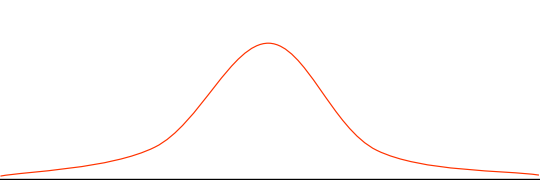
\includegraphics[width=.6\textwidth]{img/H.png}
		\end{center}
		\item G: discrete, with mass at $\phi_k$
		\begin{center}
			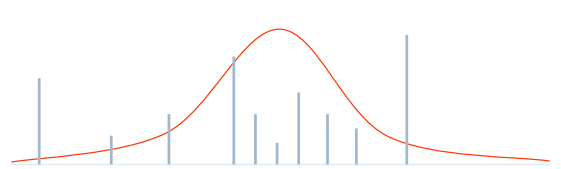
\includegraphics[width=.6\textwidth]{img/G.png}
		\end{center}
	\end{itemize}
\end{frame}

\begin{frame}
	\frametitle{An Alternative View of Mixture Model}
	\begin{itemize}
		\item Recall
		\[
			G = \sum_{k=1}^{K}\pi_k\delta_{\phi_k}
		\]
		\item Take $K \rightarrow \infty$,
		\[
			G = \sum_{k=1}^{\infty}\pi_k\delta_{\phi_k}
		\]
		\item To execute Bayesian inference, we have to find a prior for $G$
		\pause
		\item {\em Dirichlet Process}
	\end{itemize}
\end{frame}

\begin{frame}
	\frametitle{Warmup: Dirichlet Distribution}
	\begin{itemize}
		\item Dirichlet distribution is defined over $K$-dimensional probility simplex
		\[
		\Omega_K=\{(\pi_1,\ldots,\pi_K): \pi_k\ge 0,\sum_k \pi_k =1 \}
		\]
		\item We say $(\pi_1,\ldots,\pi_K)$ is Dirichlet distributed with parameters $(\alpha_1, \ldots, \alpha_K)$, if
		\[
		p(\pi_1,\ldots,\pi_K)=\frac{\Gamma(\sum_k \alpha_k)}{\prod_k \Gamma(\alpha_k)}\prod_k \pi_k^{\alpha_k-1}
		\]
	\end{itemize}
\end{frame}

\begin{frame}
	\frametitle{Warmup: Dirichlet Distribution}
	\begin{itemize}
		\item {Aggregation Property:}
		If \[
			(\pi_1,\ldots,\pi_i, \pi_{i+1},\ldots, \pi_K) \sim \text{Dirichlet}(\alpha_1,\ldots,\alpha_i, \alpha_{i+1}, \ldots, \pi_k) 
		\]
		Then
		\[
		(\pi_1,\ldots,\pi_i+\pi_{i+1},\ldots, \pi_K) \sim \text{Dirichlet}(\alpha_1,\ldots,\alpha_i+ \alpha_{i+1}, \ldots, \pi_k) 
		\]
	\end{itemize}
\end{frame}

\begin{frame}
	\frametitle{Warmup: Dirichlet Distribution}
	\begin{itemize}
		\item {Converse of Aggregation Property:}	If 
		\begin{align*}
		(\pi_1,\dots, \pi_k) & \sim \text{Dirichlet}(\alpha_1, \ldots, \pi_K) \\
		t & \sim \text{Beta}(\alpha_i \beta, \alpha_i (1-\beta)) \\
		(aka (t, 1-t) &\sim \text{Dirichlet}(\beta\alpha_i , (1-\beta)\alpha_i ))
		\end{align*}
		Then
		\begin{align*}
		& (\pi_1,\ldots,t\pi_i,(1-t)\pi_i\ldots, \pi_K) \\
		& \sim \text{Dirichlet}(\alpha_1,\ldots,\beta\alpha_i, (1-\beta)\alpha_{i+1}, \ldots, \alpha_K) 
		\end{align*}
	\end{itemize}
\end{frame}
\begin{frame}
	\frametitle{Warmup: Dirichlet Distribution}
	\begin{itemize}
		\item {Dirichlet-Multinomial conjugacy:}	If 
		\begin{align*}
		(\pi_1,\dots, \pi_K) & \sim \text{Dirichlet}(\alpha_1, \ldots, \pi_K) \\
		z & \sim Multinomial(\pi_1,\dots, \pi_K) \\
		\end{align*}
		Then
		\[
		(\pi_1,\dots, \pi_k)|z \sim \text{Dirichlet}(\alpha_1+\delta_z(1), \ldots, \pi_K+\delta_z(K))
		\]
	\end{itemize}
\end{frame}

\subsection{Definition}
\begin{frame}
	\frametitle{Dirichlet Process}
	\begin{itemize}
		\item Starting from $\pi$, slice the space finer and finer, what do we get?
		\begin{align*}
			(\pi) & \sim Dirichlet(\alpha) \\
			(\pi_1, \pi_2) & \sim Dirichlet(\alpha_1, \alpha_2) \\
			(\pi_{11},\pi_{12}, \pi_{21}, \pi_{22}) & \sim Dirichlet(\alpha_{11},\alpha_{12}, \alpha_{21},\alpha_{22}) \ldots 
		\end{align*}
		\item Because the dividing schema is arbitrary, finnally, any finite partition of $\pi$ should follow Dirichlet distribution.
		\pause
		\item Dirichlet Process is a generalization of Dirichlet distribution to infinite many components -- Recall Gaussian Process and multivariate Gaussian distribution.
	
	\end{itemize}
\end{frame}

\begin{frame}
	\frametitle{Dirichlet Process}
	\begin{itemize}
		\item Let $G$ be a probability measure over $\Omega$. For any mesearable subset $A\subset \Omega$, $G(A)=p(x\in A), x\in \Omega$
		\item Dirichlet process (DP) is a distribution over $G$. 
		\item We write 
		\[
			G \sim \text{DP}(\alpha, H)
		\]
		if for any finite partition $(A_1, \ldots, A_n)$ of $\Omega$,
		\[
			(G(A_1), \ldots, G(A_n)) \sim \text{Dirichlet}(\alpha H(A_1), \ldots, \alpha H(A_n))
		\]
		\item $H$ is the {\color{red} base distribution}
		\[
		\text{E}(G(A)) = H(A)
		\]
		\item $\alpha$ is the {\color{red} concentration parameter}
		\[
		\text{Var}(G(A)) = \frac{H(A)(1-H(A))}{\alpha+1}
		\]
	\end{itemize}
\end{frame}

\begin{frame}
	\frametitle{Dirichlet Process}
	\begin{itemize}
		\item{Our definition is all about properties of DP. How to construct a concrete sample from DP?}
		\item{Why is DP useful for clustering?}
		\item{We'll see later}
	\end{itemize}
\end{frame}

\begin{frame}
	\frametitle{Posterior Dirichlet Process}
	\begin{itemize}
		\item We'll need the posterior Dirichlet Process later
		\item Suppose $G \sim DP(\alpha, H)$, $\theta \sim G$
		\item What is $p(\theta)$ and $G|\theta$?
		\pause
		\item For any $\theta \in A \subset \Omega$, \[
			p(A)=\int_G G(A)p(G)\diff G = H(A)
		\]
		\item So $\theta \sim H$
		
	\end{itemize}
\end{frame}

\begin{frame}
	\frametitle{Posterior Dirichlet Process}
	\begin{itemize}

		\item Using dirichlet-multinomial conjugacy, for any partition $(A_1, \ldots, A_n)$,
		\begin{align*}
		& (G(A_1), \ldots, G(A_n))|\theta \\
		\sim & \text{Dirichlet}(\alpha H(A_1)+\delta_{\theta}(A_1), \ldots, \alpha H(A_n)+\delta_{\theta}(A_n))
		\end{align*}
		where $\delta_{\theta}(A)=1$ iff. $\theta \in A$
		\pause
		\item So 
		\[
		G|\theta \sim DP(\alpha+1, \frac{\alpha H + \delta_{\theta}}{\alpha+1})
		\]		
		\item We will construct a sample from DP based on the posterior
	\end{itemize}
\end{frame}

\subsection{Stick Breaking Construction}
\begin{frame}
	\frametitle{Stick Breaking Construction}
	\begin{itemize}
		\item Sample $\theta_1$ from $H$
		\item { Consider partition $(\theta_1, \Omega - \{\theta_1\}) $}
		\[
			(G(\theta_1), G(\Omega - \{\theta_1\}))|\theta_1 \sim \text{Dir}(\alpha H(\theta_1)+1, \alpha H(\Omega - \{\theta_1\}))
		\]
		\item Noting that $G(\Omega - \{\theta_1\}) = 1-G(A_1)$, $H(\theta)=0$, $H(\Omega)=1$, we get
		\[
			G(\theta_1) \sim \text{Beta}(1, \alpha)
		\]
		\item Let $\beta_1 = G(\theta_1)$
		\[
			G = \beta_1 \delta_{\theta_1} + (1-\beta_1)G_1
		\]
		where $G_1$ is a renomalized probability measure on $\Omega - \{\theta_1\}$
	\end{itemize}
\end{frame}
\begin{frame}
	\frametitle{Stick Breaking Construction}
\begin{columns}
	\column{.6\textwidth}
	\begin{itemize}
		\item {Continue the process}
		\begin{align*}
			G & =\beta_1 \delta_{\theta_1} + (1-\beta_1)G_1 \\
			G & =\beta_1 \delta_{\theta_1} + (1-\beta_1)(\beta_2 + (1-\beta_2)G_2) \\
			& \vdots \\
			G &= \sum_{k=1}^{\infty} \pi_k \delta_{\theta_k}
		\end{align*}
		where 
		\begin{align*}
		\beta_k & \sim \text{Beta}(1, \alpha) \\
		\pi_k & = \beta_k \prod_{i=1}^{k-1} (1-\beta_i) \\
		\theta_k & \sim H
		\end{align*}		
	\end{itemize}
	\column{.4\textwidth}
	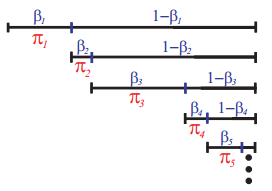
\includegraphics[width=\textwidth]{img/stick.png}
\end{columns}
\end{frame}

\begin{frame}
	\frametitle{Stick Breaking Construction}
	\begin{itemize}
		\item The above process is called the {\em stick breaking construction}
		\item What can we find about DP from this construction?
		\begin{itemize}
		\pause
		\item A sample $G$ from DP is {\color{red}discrete} with probability 1
		\pause
		\item If we keep sampling from $G$, we'll get more and more {\color{red}repeated} values
		\pause
		\item That's reasonable for clustering (why?)
		\end{itemize}
	\end{itemize}
\end{frame}

\subsection{Blackwell-MacQueen Urn Scheme}
\begin{frame}
\frametitle{Blackwell-MacQueen Urn Scheme}
	\begin{itemize}
		\item{But for clustering, we're actually interested in sampling mixture parameters $\theta_1, \theta_2, \ldots$ from $\Omega$, integrating $G$ out.}
		\pause
		\item It seems easy. $\theta_1, \theta_2, \ldots, \theta_n$ are independent given G. So we can simply sample each $\theta$ from $H$ independently, right?
		\pause
		\item No! $\theta$s are no longer indenpendent if we integrate $G$ out
		\[
		p(\theta_1, \theta_2, \ldots, \theta_n) = \int_G \prod_{i=1}^{n} p(\theta_i|G)p(G) \diff G
		\]
	\end{itemize}
\end{frame}
\begin{frame}
	\frametitle{Blackwell-MacQueen Urn Scheme}
	\begin{itemize}
		\item Consider two samples $\theta_1, \theta_2$.
		\begin{align*}
		p(\theta_2 | \theta_1) & = \int_G \prod_{i=1}^{n} p(\theta_2, G| \theta_1) \diff G \\
		& = \int_G \prod_{i=1}^{n} p(\theta_2|G) p(G|\theta_1) \diff G 
		\end{align*}
		\item We have already known the posterior distribution of $G$ given $\theta_1$,
		
		\[
		G|\theta_1 \sim \text{DP}(\alpha+1, \frac{\alpha H + \delta_{\theta_1}}{\alpha+1})
		\]
		\item Then, given $\theta_1$, the second sample $\theta_2$ can be sampled from the posterior base distribution.
		\item The sampling process becomes quite simple		
	\end{itemize}
\end{frame}
\begin{frame}
	\frametitle{Blackwell-MacQueen Urn Scheme}
	\begin{itemize}
		\item First sample: 
			\[ \theta_1 \sim H, \quad G|\theta_1 \sim \text{DP}(\alpha+1, \frac{\alpha H + \delta_{\theta_1}}{\alpha+1}) \]
		\item Second sample:
			\[ \theta_2|\theta_1 \sim \frac{\alpha H + \delta_{\theta_1}}{\alpha+1}, \quad G|\theta_1,\theta_2 \sim \text{DP}(\alpha+2, \frac{\alpha H + \delta_{\theta_1} + \delta_{\theta_2}}{\alpha+2}) \]
		\item $n^{th}$ sample:
			\[ \theta_n|\theta_{1,\ldots,n-1} \sim \frac{\alpha H + \sum_{k=1}^{n-1}\delta_{\theta_k}}{\alpha+n-1}, \quad G|\theta_{1,\ldots,n} \sim \text{DP}(\alpha+n, \frac{\alpha H + \sum_{k=1}^{n}\delta_{\theta_k}}{\alpha+n}) \]
	\end{itemize}
\end{frame}

\begin{frame}
	\frametitle{Blackwell-MacQueen Urn Scheme}
	\begin{itemize}
		\item One issue, how to sample from $\frac{\alpha H + \sum_{k=1}^{n-1}\delta_{\theta_k}}{\alpha+n-1}$?
		\begin{itemize}
			\item With probability $\propto \alpha$, sample from $H$
			\item With probability $\propto n-1$, randomly pick one from $\theta_1,\ldots,
			 \theta_{n-1}$
		\end{itemize}
		\item The above sample process is called {\em Blackwell-MacQueen Urn Scheme}
		\item Samples $\theta_1, \ldots, \theta_n$ induces a partition over $1,\ldots,n$, if we cluster repeated values together
		\item Working with float value is annoying. We can postpone sampling from $H$ -- {\color{red}Chinese Restaurant Process}
	\end{itemize}
\end{frame}

\subsection{Chinese Restaurant Process}
\begin{frame}
\frametitle{Chinese Restaurant Process}
	\begin{itemize}
		\item Generating process of CRP:
		\begin{itemize}
			\item First customer sits at the first table.
			\item $n^{th}$ customer
				\begin{itemize}
					\item With probability $\frac{n_k}{\alpha+n-1}$, sits at existing table $k$, where $n_k$ is number of customers at table $k$.
					\item With probability $\frac{\alpha}{\alpha+n-1}$, sits at a new table $K+1$, where $K$ is number of existing tables.
				\end{itemize}
		\end{itemize}
		
		\item CPR teases apart clustering properity of DP from base distribution $H$
		\item To get back to Blackwell-MacQueen Urn Scheme, sample $\theta_k$ for each table $k$
	\end{itemize}
\end{frame}

\begin{frame}
	\frametitle{CRP and DP}
	\begin{itemize}
		\item We can prove that the order of customer coming in doesn't affect partition probability
		\item Infinite Exchangeability:
			\[
			\forall n, \forall \sigma, p(x_1, \ldots, x_n)=p(x_{\sigma(1)},\ldots, x_{\sigma(n)})
			\]
		\item De Finetti’s Theorem: If $(x_1, x_2, \ldots)$ are infinite exchangable, then there exists a random variable $\theta$, $\forall n$, 
			\[
			 p(x_1, \ldots, x_n) = \int_{\theta} \prod_{i=1}^n p(x_i|\theta)p(\theta) \diff \theta
			\]		
		\item Here, DP is the distribution of $\theta$	
	\end{itemize}
\end{frame}

\begin{frame}
	\frametitle{CRP and Clustering}
	\begin{itemize}
		\item We can view {\em data points} as customers, {\em clusters} as tables.
		\item CRP defines a prior distribution on partition (cluster) of data. Number of clusters can be induced
		\item Combined with a parameterized probability distribution for each cluster, we can get a posterior
		\item That's all we need in cluster settings
	\end{itemize}
\end{frame}

\subsection{DP Mixture Inference}

\begin{frame}
	\frametitle{Gibbs Sampling DP Mixtures}
	\begin{itemize}
		\item Go back to original Gaussian Mixture clustering model. Let's place $DP(\alpha,H)$ as prior of $G$ -- DP mixture
		\item Introduce $z_i$ as cluster indicator for each $x_i$
		\item We use {\color{red} collapsed} Gibbs sampling for inference
		\[
			p(z_i=k|\bm{z}_{-i},\bm{x},\bm{\nu},\alpha) \propto p(z_i=k|\bm{z}_{-i}, \alpha)p(x_i|\bm{x}_{-i}, z_i=k, \bm{z}_{-i}, \bm{\nu})
		\]
		where \[
			p(z_i=k|\bm{z}_{-i}, \alpha) = \frac{n_k}{\alpha+n-1}
		\] for existing component $k$ among $\bm{z}_{-i}$, and 
		\[
			p(z_i=K|\bm{z}_{-i}, \alpha) = \frac{\alpha}{\alpha+n-1}
		\] for new component $K+1$, $\forall j \neq i, z_j \neq K+1$
	\end{itemize}
\end{frame}

\begin{frame}
	\frametitle{Gibbs Sampling for DP Mixtures}
	\begin{itemize}
		\item What is $p(x_i|\bm{x}_{-i}, z_i=k, \bm{z}_{-i}, \bm{\nu})$ ?
		\item For new component $K+1$, $x_i$ is conditional indenpendent from other data points
		\[
		p(x_i|\bm{x}_{-i}, z_i=K+1, \bm{z}_{-i}, \bm{\nu})
		= \int_{\phi} p(x_i|\phi)p(\phi | \nu) \diff \phi
		\]
		\item For existing component $k$, $x_i$ is conditional indenpendent from data points in different cluster
		\[
		p(x_i|\bm{x}_{-i}, z_i=k, \bm{z}_{-i}, \bm{\nu})
		= \frac{p(x_i, \bm{x}_{-i}^{(k)}|\nu)}{p(\bm{x}_{-i}^{(k)}|\nu)}
		\]		
		It's model specific.
	\end{itemize}
\end{frame}
\begin{frame}
	\frametitle{Visulization}
	\centering{
	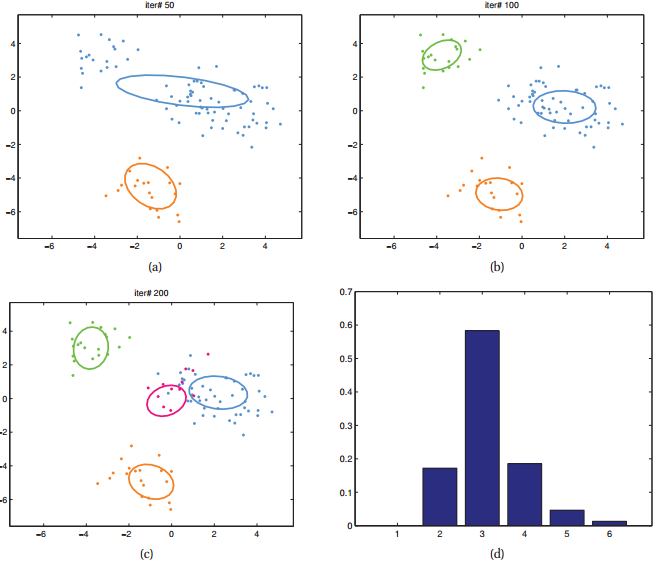
\includegraphics[width=0.7\textwidth]{img/dpmixture.png}
	}
\end{frame}
\begin{frame}
	\frametitle{Other methods}
	\begin{itemize}
		\item I don't like sampling. Is there any analytic method?
		\item Based on the stick-breaking construction, we have a variational method.
		\item But we won't cover it here.
	\end{itemize}
\end{frame}

\end{document}